\chapter{Preliminaries}\label{chap:preliminaries}

\section{SAT basics}

\subsection{Satisfiability problem}
A \emph{Boolean variable}, or \emph{propositional variable}, is a variable that
has two possible values : true or false (noted $\true$ or $\false$,
respectively).  A \emph{literal} $l$ is a propositional variable or its
negation. For a given variable $x$, the positive literal is represented by $x$
and the negative one by $\neg x$.
A \emph{clause} $\omega$ is a finite disjunction of literals represented
equivalently by $\omega = \bigvee_{i=1}^k l_i$ or the set of its literals
$\omega = \{l_i\}_{i \in \llbracket 1,k \rrbracket}$. A clause with a single
literal is called \emph{unit clause}.
A \emph{conjunctive normal form (CNF) formula} $\varphi$ is a finite
conjunction of clauses.  A CNF can be either noted $\varphi = \bigwedge_{i=1}^k
\omega_i$ or $\varphi = \{\omega_i\}_{i \in \llbracket 1,k \rrbracket}$. We
denote $\Vars_\varphi$ ($\Lits_\varphi$) the set of variables (literals) used in
$\varphi$ (the index in $\Vars_\varphi$ and $\Lits_\varphi$ is usually omitted when
clear from context).

For a given formula $\varphi$, an \emph{assignment} of the variables of
$\varphi$ is a function $\alpha: \Vars \mapsto \{ \true, \false \}$.  As usual, $\alpha$ is
\emph{total}, or \emph{complete}, when all elements of $\Vars$ have an image by
$\alpha$, otherwise it is \emph{partial}. By abuse of notation, an assignment is
often represented by the set of its true literals.  The set of all (possibly
partial) assignments of $\Vars$ is noted $\Assignments(\Vars)$.

The assignment $\alpha$ \emph{satisfies} the clause $\omega$, denoted $\alpha
\models \omega$, if $\alpha \cap \omega \neq \emptyset$. Similarly, the assignment
$\alpha$ satisfies the propositional formula $\varphi$, denoted $\alpha \models
\varphi$, if $\alpha$ satisfies all the clauses of $\varphi$. Note that a
formula may be satisfied by a partial assignment. In this case, unassigned variable are called
\emph{dont care}.
A formula is said to be
\emph{satisfiable} (\sat) if there is at least one assignment that satisfies it;
otherwise the formula is \emph{unsatisfiable} (\unsat).

\subsection{An NP-complete problem}


The SAT problems is the first NP-complete algorithm as proven by Stephen Cook in 1971~\cite{cook1971complexity}.
It is also proved by Leonid Levin in 1973~\cite{4640789}, for this purpose, it was known as Cook-Levin theorem.
The proof of to show that can be found in \cite{sipser2006introduction}.
Any NP problem can be reduced to a SAT problem in polynomial time and so open one of the most important 
unsolved problem in theoretical computer science is the P versus NP problem.
This question is one of the seven millennium prize problems.


%It asks if every problems can be solved and verified in polynomial time.
%Any NP problems can be reduced in polynomial time by a deterministic Turing machine to the SAT problems.
%The states that the propositional satisfiability problem is NP-complete
%SAT is NP because any assignment of Boolean values to Boolean variables that is claimed to 
%satisfy the given expression can be verified in polynomial time by a deterministic Turing machine. 
%
%


\subsection{Solving a SAT problem}

A naive approach to solve a SAT problem is to try all possible assignments. In total,
for a propositional formula with $n$ variables, it leads to $2^n$ assignments.  
Figure~\ref{fig:naive_algo} illustrate the search tree for a problem with six variables.
This algorithm is obviously intractable on real problems even for a formula with few variables. 
 
\begin{figure}[H]
	\centering
	
\begin{minipage}[c]{0.6\linewidth}
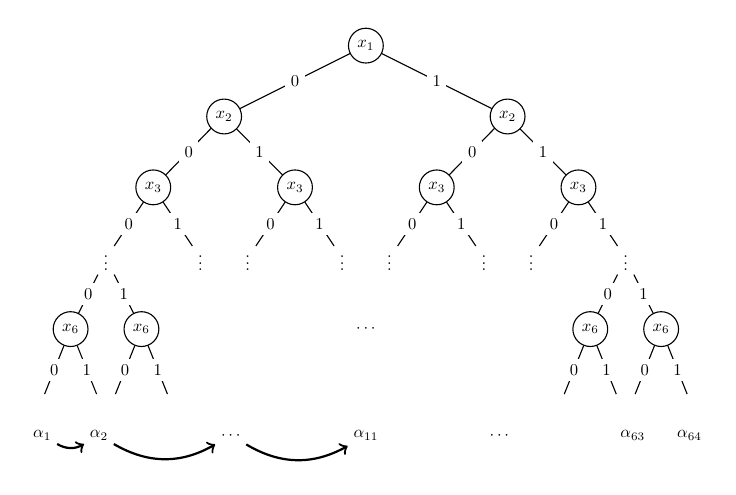
\begin{tikzpicture}[level/.style={sibling distance=60mm/#1},every node/.style={scale=0.6}, scale=0.6]
  \tikzstyle{trans}=[thick, ->, sloped]

\node [circle,draw] (x1) {$x_1$}
  child {node [circle,draw] (x2_1) {$x_2$}
    child {node [circle,draw] (x3_1) {$x_3$}
      child {node  (xn_1) {$\vdots$}
        child {node [circle,draw] (x6_1) {$x_6$}
        	child {node (x6_1f) {}
        	child[level distance=0.75cm] { node (a1) {$\alpha_1$} edge from parent[draw=none]}
        }
       		child {node (x6_1t) {}
       			child[level distance=0.75cm] { node (a2) {$\alpha_2$} edge from parent[draw=none]}
         }}
        child {node [circle,draw] (x6_2) {$x_6$}
        		child {node (x6_2f) {}}
        				child {node (x6_2t) {}
        	}
        }
      } 
      child {node (xn_2) {$\vdots$}}
    }
    child {node [circle,draw] (x3_2) {$x_3$}
      child {node (xn_3) {$\vdots$}}
      child {node (xn_4) {$\vdots$}}
    }
  }
  child {node [circle,draw] (x2_2) {$x_2$}
    child {node [circle,draw] (x3_3) {$x_3$}
      child {node (xn_5) {$\vdots$}}
      child {node (xn_6) {$\vdots$}}
    }
  child {node [circle,draw] (x3_4) {$x_3$}
    child {node (xn_7) {$\vdots$}}
    child {node (xn_8) {$\vdots$}
      child {node [circle,draw] (x6_3) {$x_6$}
      	       child {node (x6_3f) {}}
      	child {node (x6_3t) {}
        }}
      child {node [circle,draw] (x6_4) {$x_6$}
      	child {node (x6_4f) {}
        child[level distance=0.75cm] { node (an_1) {$\alpha_{63}$} edge from parent[draw=none]}
    	}
	    child {node (x6_4t) {}
    		child[level distance=0.75cm] { node (an) {$\alpha_{64}$} edge from parent[draw=none]}
      }}}
  }
};

\path (x6_2) -- (x6_3) node (x) [midway] {$\cdots$}
        child[level distance=2.25cm] { node (a_11) {$\alpha_{11}$} edge from parent[draw=none]};


\path (a2) -- (a_11) node (b1) [midway] {$\cdots$};
\path (a_11) -- (an_1) node (b2) [midway] {$\cdots$};

\draw[trans] (a1) to [bend right]  (a2);
\draw[trans] (a2) to [bend right]  (b1);
\draw[trans] (b1) to [bend right]  (a_11);

% to [bend right]  (b1) to [bend right]  (a_11);

\path (x1)   -- (x2_1) node [midway, fill=white] {$0$};
\path (x2_1) -- (x3_1) node [midway, fill=white] {$0$};
\path (x3_1) -- (xn_1) node [midway, fill=white] {$0$};
\path (xn_1) -- (x6_1) node [midway, fill=white] {$0$};
\path (x3_2) -- (xn_3) node [midway, fill=white] {$0$};
\path (x2_2) -- (x3_3) node [midway, fill=white] {$0$};
\path (x2_2) -- (x3_4) node [midway, fill=white] {$1$};
\path (x1)   -- (x2_2) node [midway, fill=white] {$1$};
\path (xn_1) -- (x6_2) node [midway, fill=white] {$1$};
\path (x3_1) -- (xn_2) node [midway, fill=white] {$1$};
\path (x2_1) -- (x3_2) node [midway, fill=white] {$1$};
\path (x3_2) -- (xn_4) node [midway, fill=white] {$1$};
\path (x3_3) -- (xn_5) node [midway, fill=white] {$0$};
\path (x3_3) -- (xn_6) node [midway, fill=white] {$1$};
\path (x3_4) -- (xn_7) node [midway, fill=white] {$0$};
\path (x3_4) -- (xn_8) node [midway, fill=white] {$1$};
\path (xn_8) -- (x6_3) node [midway, fill=white] {$0$};
\path (xn_8) -- (x6_4) node [midway, fill=white] {$1$};


\path (x6_1) -- (x6_1f) node [midway, fill=white] {$0$};
\path (x6_1) -- (x6_1t) node [midway, fill=white] {$1$};

\path (x6_2) -- (x6_2f) node [midway, fill=white] {$0$};
\path (x6_2) -- (x6_2t) node [midway, fill=white] {$1$};

\path (x6_3) -- (x6_3f) node [midway, fill=white] {$0$};
\path (x6_3) -- (x6_3t) node [midway, fill=white] {$1$};

\path (x6_4) -- (x6_4f) node [midway, fill=white] {$0$};
\path (x6_4) -- (x6_4t) node [midway, fill=white] {$1$};

\end{tikzpicture}
\end{minipage}
\begin{minipage}[c]{0.23\linewidth}
           \footnotesize
		\begin{itemize}
			\item[] $\omega_1 = \{x_1, x_2, x_3\}$ 
			\item[] $\omega_2 = \{x_4, x_5, x_6\}$
			\item[] $\omega_3 = \{\neg x_1, \neg x_5\}$
			\item[] $\omega_4 = \{\neg x_2, \neg x_4\}$
			\item[] $\omega_5 = \{\neg x_3, \neg x_4\}$
			\item[] $\omega_6 = \{\neg x_3, \neg x_6\}$
		\end{itemize}
\end{minipage}

	\caption{All possible assignments for a problem with 6 variables}
	\label{fig:naive_algo}
\end{figure}

%\hakan{Parler du DP}

One of the first non memory intensive algorithm to solve the SAT problems is 
the Davis Putnam Logemann Loveland (DPLL) algorithm~\cite{dpll_62}. 
This algorithm introduces the \emph{unit propagation}.
This principle force the value of a literal when a clause is \emph{assertive}, i.e. 
has all literals to false but one unassigned. It will force the value of the unassigned literal 


The iterated application of unit propagation until a fix point is called \emph{unit propagation} or \emph{boolean constraint propagation } (BCP).

Another idea introduced by DPLL was \emph{elimination of pure literals},
a literal is said pure if it only appear on one sign (positive or negative) in the problem.
These literals are set to true in the assignment.
On consequence, all clauses that own these literals are satisfied and so can be removed.

A conflict 



Another sound and complete algorithm to resolve a SAT problem is 
Conflict-Driven Clause learning (CDCL) algorithm~\ref{algo:cdcl} and is inspired DPLL.
This algorithm introduces two principles. The first one is \emph{no chronological backtracking}



The CDCL algorithm walks a binary search tree.  It first applies unit propagation to
the formula $\varphi$ for the current assignment $\alpha$ (line~\ref{alg:cdcl:unit}).
A conflict at level $0$ indicates that the formula is not satisfiable, and the algorithm
reports it (lines~\ref{alg:cdcl:unsat_start}-\ref{alg:cdcl:unsat_end}).
If a conflict is detected, it is analyzed, which provides a \emph{conflict clause} 
explaining the reason for the conflict (line~\ref{alg:cdcl:analyze}).
Different heuristics exists about the computation of conflict clause, on recent solvers
the most used heuristic is the first Unique Implication Point ($1^{th}$ UIP) \cite{zhang2001efficient}.
The analysis is completed by the computation of a
backjump point to which the algorithm backtracks (line~\ref{alg:cdcl:backjump}).
Restart is an important things in SAT solver, it allows solver to explore a new search space
with the learned clauses. It is also finely intertwined with the decision heuristics.
If the solver is working on "hard" part of the problem it will reconsider the decision variables and
solve this part part at first. But if we restart too often the solver doesn't have to discover new things.

  This clause is learnt (line~\ref{alg:cdcl:learn}), as it does not change the
satisfiability of $\varphi$, and avoids encountering a conflict with the same
causes in the future.
Finally, if no conflict appears, the algorithm chooses a new decision literal 
(line~\ref{alg:cdcl:pick_start}-\ref{alg:cdcl:pick_end}). The choice of the decision literal
affect the performance of solver. The first most used heuristic is Variable State Independent Decaying Sum (VSIDS)~\cite{moskewicz2001chaff}. The idea behind this heuristic is that the "hard" parts of the search space 
will be treated first. To do that, each variable has an activity and wa increase if it participate to the resolution
of the conflict.
The second most used heuristics is Learning rate based branching (LRB~\cite{liang2016learning})
The above steps are repeated until the satisfiability status of the formula is determined.


\begin{algorithm}
	\SetKwProg{Fn}{function}{}{}
	\SetKwFunction{CDCL}{CDCL}
	\SetKwFunction{unitPropagation}{unitPropagation}
	\SetKwFunction{analyzeConflict}{analyzeConflict}
	\SetKwFunction{addLearntClause}{addLearntClause}
	\SetKwFunction{assignNewLiteral}{assignDecisionLiteral}
	\SetKwFunction{backjumpPolicy}{backjumpAndRestartPolicies}
	\SetKwFunction{ca}{currenttAssignment}
	\Fn{
		\CDCL{$\varphi$: CNF formula}\\
		$\quad\quad$\textbf{returns} $\true$ if $\varphi$ is \sat and $\false$ otherwise
	}
	{
		$dl \gets 0$ \tcp*{Current decision level}
		\While{not all variables are assigned}{
			$isConflict \gets$ \unitPropagation{}\;\label{alg:cdcl:unit}
			\If{$isConflict$}{
				\If{dl = 0}{\label{alg:cdcl:unsat_start} 
					\Return \false \label{alg:cdcl:unsat_end} 
					\tcp*{$\varphi$ is $\unsat$}
				}
				$\omega \gets$ \analyzeConflict{}\;\label{alg:cdcl:analyze} 
				$dl \gets$ \backjumpPolicy{}\;\label{alg:cdcl:backjump} 
				$\varphi \gets \varphi \cup \{\omega$\} \; \label{alg:cdcl:learn}
				
			}
			\Else{
				\assignNewLiteral{}\; \label{alg:cdcl:pick_start} 
				$dl \gets dl+1$\;\label{alg:cdcl:pick_end} 
			}
		}
		\Return \true
		\tcp*{$\varphi$ is $\sat$}
	}
	\caption{The CDCL algorithm.}
	\label{algo:cdcl}
	
\end{algorithm}


\hakan{Peut être mettre les heuristiques dans des paragraphes}

\hakan{Literal Block Distance LBD}

\section{Groups basics}

Symmetries is related to a branch of mathematics called group theory. This section give us an overview of group
theory.

\subsection{Groups}

A \emph{group} is a structure $\langle G, * \rangle$, where $G$ is a non empty set and $*$ a binary
operation such the following axioms are satisfied:
\begin{itemize}[noitemsep,nolistsep]
	\item \emph{associativity}: $\forall a, b, c \in G, (a * b) * c = a * (b * c)$
	\item \emph{closure}: $\forall a, b \in G, a * b \in G$.
	\item \emph{identity}: $\forall a \in G, \exists e$ such that $ a * e = e * a = a$
	\item \emph{inverse}:  $\forall a \in G, \exists b \in G$, commonly denoted $a^{-1}$ such that
	 $a * a^{-1} = a^{-1} * a = e$
\end{itemize}

Note that \emph{commutativity} is not required i.e $\ a * b = b * a$, for $a, b \in G$.
The group is \emph{abelian} if it satisfies the commutativity rule.
Moreover, the last definition leads to important properties which are: i) uniqueness of the identity element. 
To prove this property, assume $\langle G, * \rangle$ a group with two identity elements $e$ and $f$ 
then $ e = e * f = f$.
ii) uniqueness of the inverse element. To prove this property, suppose that an element $x_1$ has two inverses,
denoted $b$ and $c$ in group $\langle G, * \rangle$, then\\
	$\begin{array}{lcll}					
			b & = & b * e & \\
			  & = & b * (a * c) & c \text{ is an inverse of } a, \text{so } e = a * c\\
			  & = & (b * a) * c &   \text{\emph{associativity} rule}\\
			  & = & e * c       & b \text{ is an inverse of } a, \text{so } e = a * b\\
			  & = & c           &   \text{\emph{identity} rule}
	\end{array}$

The structure $\langle G, * \rangle$ is denoted as G when clear from context that G is a group
with a binary operation. In this thesis, we interested only with the \emph{finite} groups i.e
with a finite number of elements.

Given a group $G$, a \emph{subgroup} is a non empty subset of $G$ which is also a group with 
the same binary operation. If $H$ is a subgroup of $G$, we denote as $H \leq G$.
A group has at least two subgroups: i) the subgroup composed by identity element $\{e\}$, denoted \emph{trivial} subgroup. All other subgroups are \emph{nontrivial}; ii) the subgroup composed by itself, denoted \emph{improper} subgroup. All other subgroups are \emph{proper}.


\subsubsection{Generators of a group}

If every elements in a group G can be expressed as a linear combination
of a set of group of elements S = $\{g_1, g_2, ..., g_n \}$ then we say G is 
generated by the S. we denote this as G = $\langle S \rangle$ =
$\langle \{g_1, g_2, ..., g_n \} \rangle$ 



\subsection{Permutation groups}
 
A \emph{permutation} is a bijection from a set $X$ to itself.\\
 Example: given a set $X = \{x_1, x_2, x_3, x_4, x_5, x_6\}$,
$g = ${\Bigg( \begin{tabular}{cccccc}
		$x_1$ & $x_2$ & $x_3$ & $x_4$ & $x_5$ & $x_6$\\
		$x_2$ & $x_3$ & $x_1$ & $x_4$ & $x_6$ & $x_5$
	\end{tabular} \Bigg)}\\
$g$ is a permutation that maps $x_1$ to $x_2$, $x_2$ to $x_3$, $x_3$ to $x_1$, $x_4$ to $x_4$, $x_5$ to $x_6$ and $x_6$ to $x_5$.

Permutations are generally written in \emph{cycle notation} and the self mapped elements are omitted.
So the permutation in cycle notation will be : $g$ = ($x_1$ $x_2$ $x_3$) ($x_5$ $x_6$).
We say \emph{support} of the permutation $g$ noted $supp(g)$ the elements that not mapped to themselves,
$supp(g) = \{ x \in X \mid g.x \neq x\}$. A variable $x$ is \emph{stabilized} by a permutation $g$ 
if $x \notin \support(g)$. A clause $\omega$ is \emph{stabilized} by a permutation $g$ if 
$\omega \cap \support(g) = \emptyset$. \hakan{Maybe stabilisation as definition ?}


The set of permutations of a given set $X$ form a group $G$,
with the composition operation ($\circ$) and called \emph{permutation group}.
The \emph{symmetric group} id the set of all possible permutations of a set $X$ and noted \Group($X$).
%The set of \textbf{all} permutations of a set $X$ is the \emph{symmetric group} of $X$ and noted \Group($X$).
So, a \emph{permutation group} is a subgroup of \Group($X$). 
%A set of permutations $P$ is a set of \emph{generators} of a group $G$ if each permutation of $G$
%can be expressed as a composition of permutations in $P$. 


A permutation group $G$ induces a \emph{equivalence relation} on the set of element $X$ being
permuted. Two elements $x_1, x_2 \in X$ are equivalent if there exists a permutation $g \in G$ such that
$g x_1 = x_2$. Then equivalence relation partitions $X$ into \emph{equivalence classes} referred to
as the \emph{orbits} of $X$ under $G$. The orbit of an element $x$ under group $G$ (or simply orbit of $x$ when clear
from the context) is the set $[x]_G = \{g.x \mid g \in G\}$




